\documentclass[12pt,a4paper]{article}
\usepackage{physics}
\usepackage{amssymb}
\usepackage{subcaption}
\input{spp.dat}

%  Editorial staff will uncomment the next line
% \providecommand{\artnum}[0]{XX-XX}
% \renewcommand{\articlenum}[0]{SPP-\the\year-\artnum-}

\begin{document}

\title{\TitleFont Activity 2 -- Practical Image Processing 2}
\author[ ]{\textbf{Kenneth V. Domingo} \\
2015--03116 \\
App Physics 186, 1\textsuperscript{st} Semester, A.Y. 2019--20}
\affil[ ]{\corremail{kvdomingo@up.edu.ph} }

\maketitle
\thispagestyle{titlestyle}

\section*{Results and Discussion}
Today's activity involved the basics on digitally extracting values from hand-drawn plots. The image I used is shown in Fig. \ref{fig:plot-used}. For the pixel coordinate extraction, I used Photoshop, and for everything else, Python's \texttt{matplotlib} module.

\begin{figure}[!htb]
	\centering
	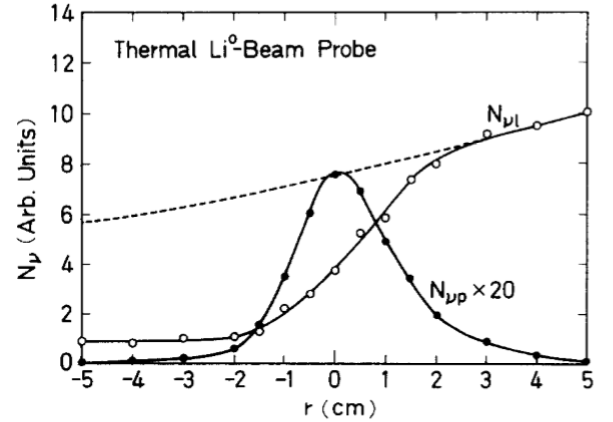
\includegraphics[width=0.6\textwidth]{graph-image.png}
	\caption{Radial profiles of the electron excitation emission $N_{\nu p}$ and the laser-induced fluorescence $N_{\nu l}$ for lithium resonance line (670.8 nm) \cite{kadota}.}	
	\label{fig:plot-used}
\end{figure}

In order to determine the pixel-to-centimeter conversion factor, I first tabulated the pixel coordinates of the $x$-- and $y$--axis units. I noticed that the ticks were not equidistant, and that the $x$ and $y$ axes were not of the same scale, so I performed linear regression by plotting the pixel vs cm values separately for both axes. The calibration curves can then be obtained from Fig. \ref{fig:calib}.

\begin{figure}[!htb]
	\centering
	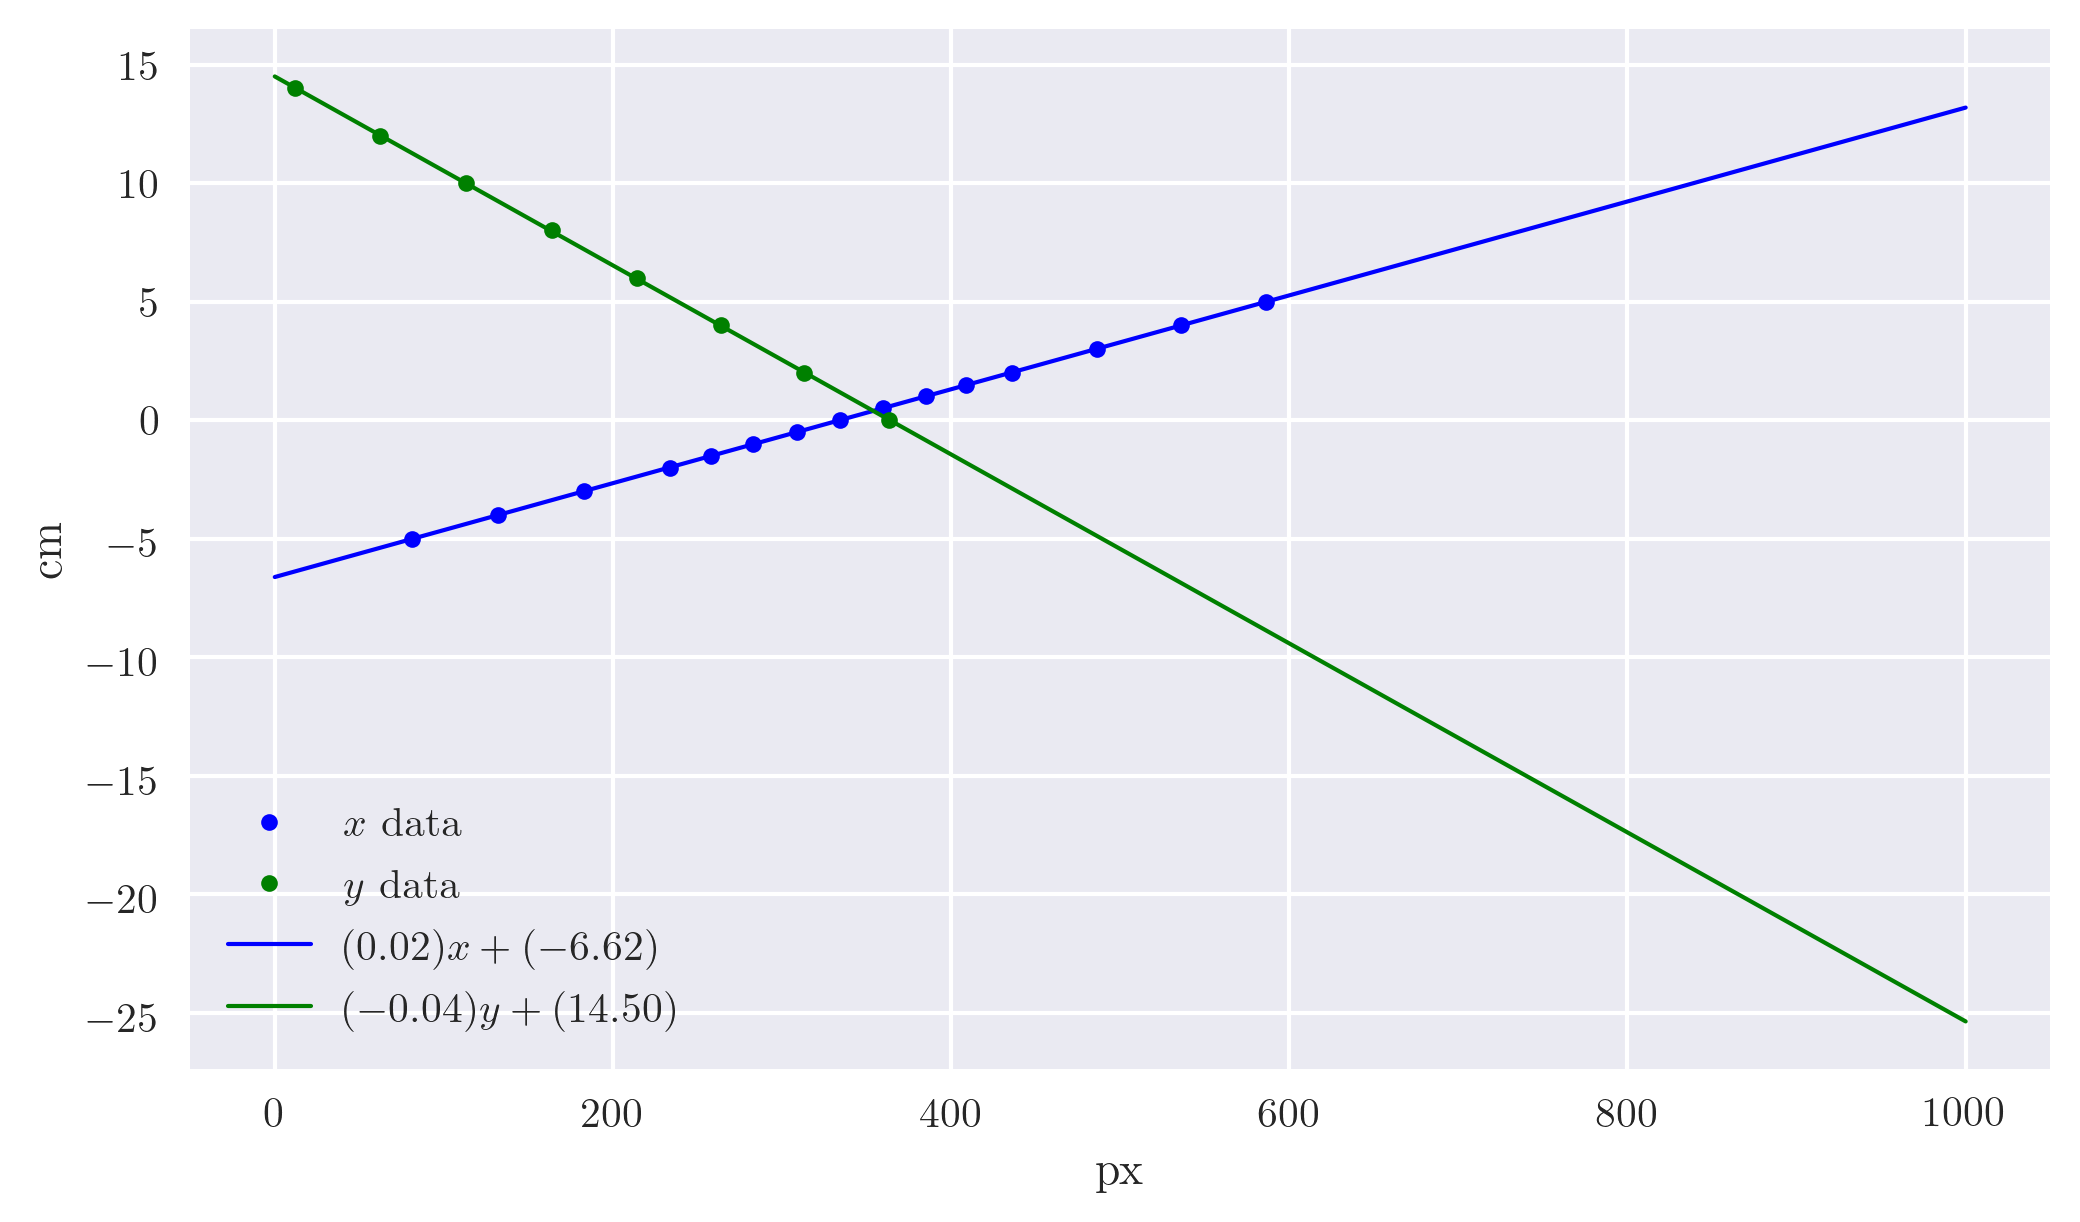
\includegraphics[width=0.9\textwidth]{calibration_curves.png}
	\caption{Calibration curves for the $x$ and $y$ axes.}	
	\label{fig:calib}
\end{figure}

The conversion factors obtained were:

\begin{align}
	x_{cm} &= (0.02)x_{px} - 6.62 \label{eq:calibx} \\
	y_{cm} &= (-0.04)y_{px} + 14.50 \label{eq:caliby}
\end{align}

Using these conversion factors, it's simply a matter of plugging in pixel values into \eqref{eq:calibx} or \eqref{eq:caliby} in order to extract the real cm units. In Fig. \ref{fig:plot-used}, we can see three elements: a bell curve, a sigmoid-like curve, and an apparently straight line (it actually curves ever so slightly upward). To extract the values of the bell curve, I simply took the pixel location of the center of the round markers. For the sigmoid, I sampled at points on the line immediately adjacent to the hollow markers. For the dashed line, I sampled at each $x$-axis unit.

After performing the necessary conversions, I could then plot my extracted curves while overlaying original image all in one go. Because \texttt{matplotlib}'s \texttt{imshow} function displays images in terms of pixels, I had to specify its \texttt{extent} and \texttt{aspect} parameters. To do this, I have to determine the length and width of the image as a whole, i.e., I have to extend the axes of the original plot so that it encompasses the image as a whole. This task is already trivial since I have already calculated conversion factors earlier. The end product is shown in Fig. \ref{fig:output}.

\begin{figure}[!htb]
	\centering
	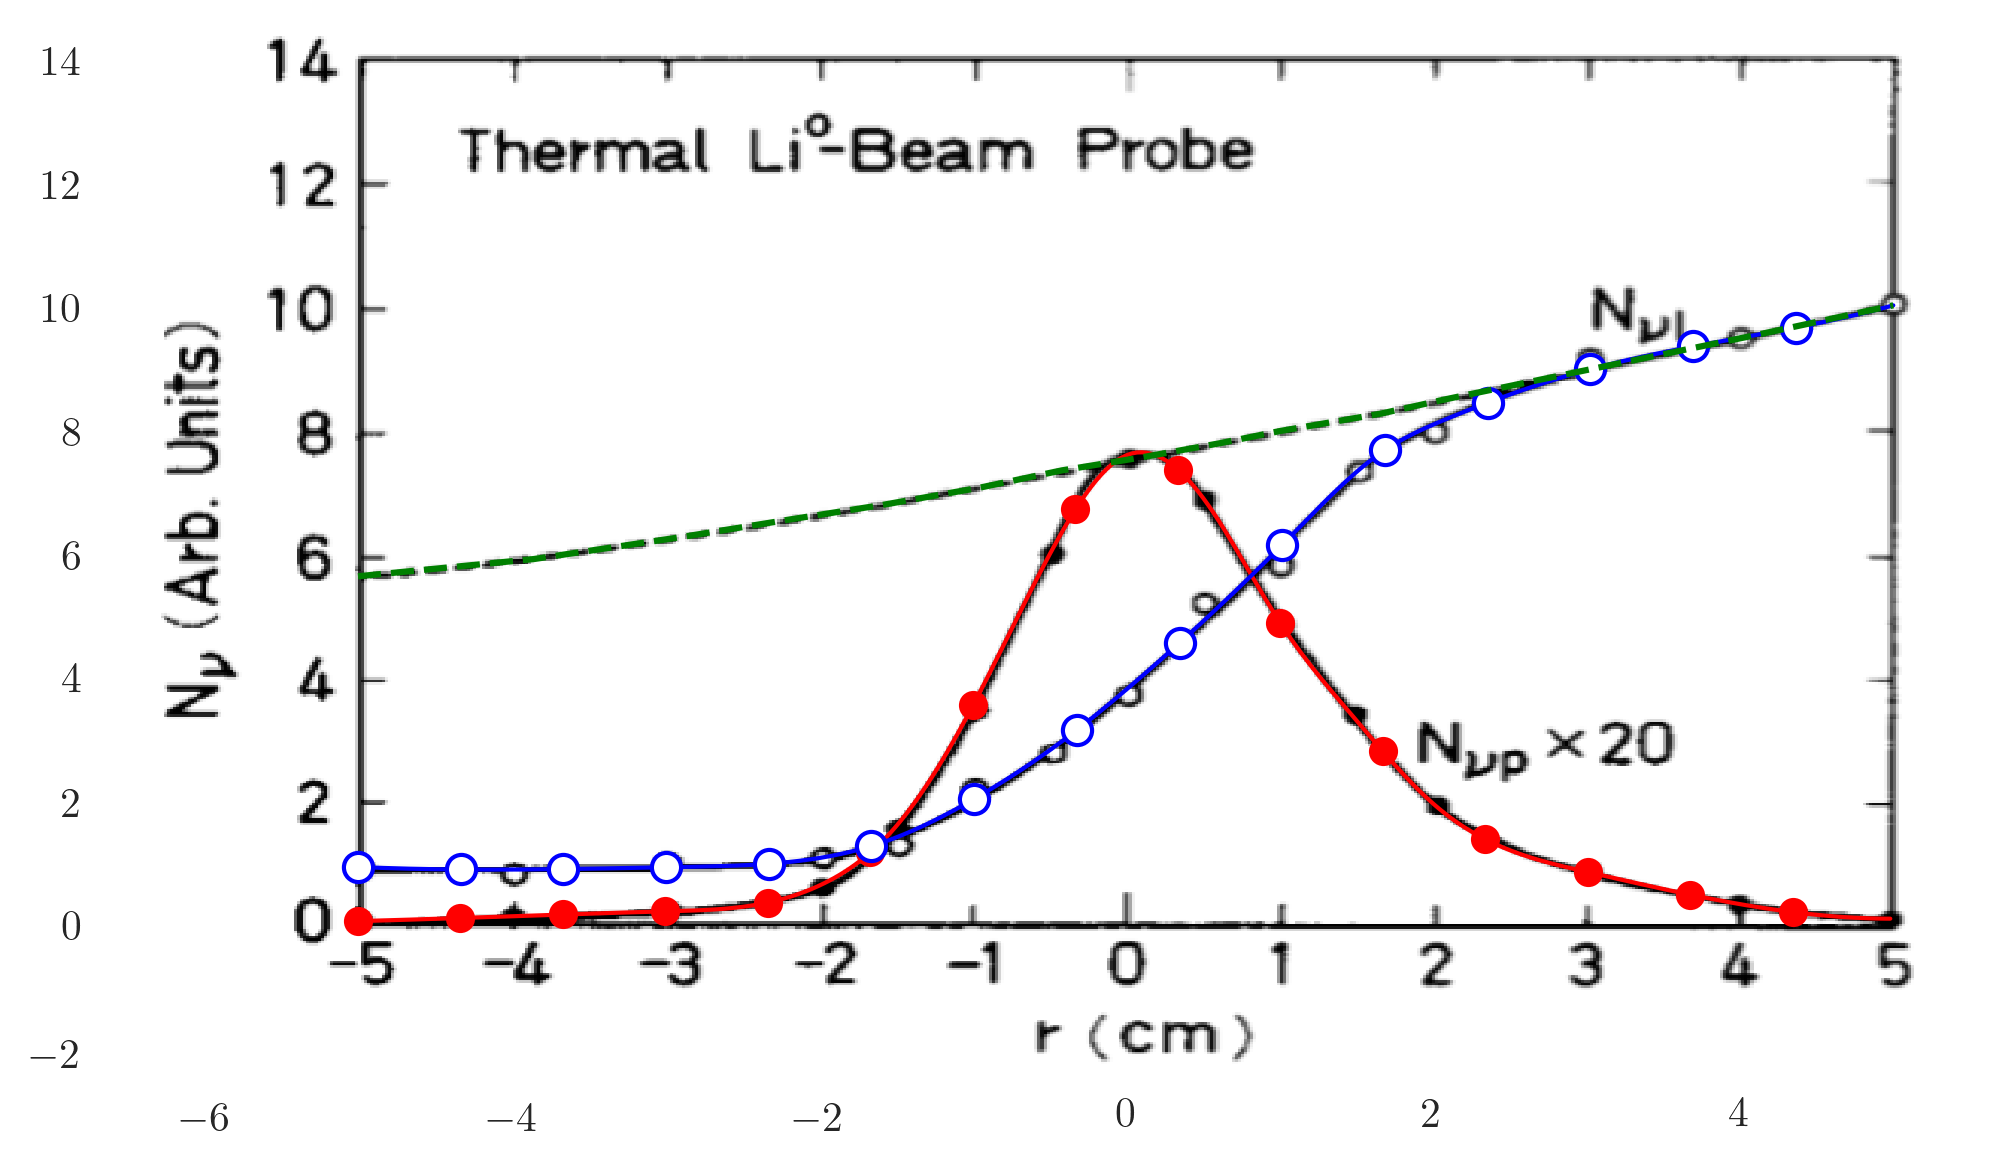
\includegraphics[width=0.9\textwidth]{final_overlay.png}
	\caption{Original image overlayed with the extracted curves.}	
	\label{fig:output}
\end{figure}

Even though it was suggested to use Paint, GIMP, and/or a spreadsheet software, I opted to use Photoshop and \texttt{matplotlib} since I have been accustomed to using them and I believe I can work faster and more efficiently by using them. Personally, I find using Excel cumbersome and \textit{makalat tignan} for data processing, and I am especially not fond of the appearance of its plots.

\begin{table}[!htb]
	\centering
	\caption{Self-evaluation.}
	\begin{tabular}{|r|c|}
		\hline
		Technical correctness & 5 \\ \hline
		Quality of presentation & 5 \\ \hline
		Initiative & 1 \\ \hline
		\textbf{TOTAL} & \textbf{11} \\ \hline
	\end{tabular}
	\label{tab:self-eval}
\end{table}


\bibliographystyle{spp-bst}
\bibliography{186-Act2}

\end{document}